\chapter{Felhasználói dokumentáció}
\label{ch:user}

A következő fejezetben fogom bemutatni az alkalmazás elérését, egyes komponenseit, illetve felhasználási lehetőségeit. 

Ez a pénzügyeket rendszerező alkalmazás alapvetően magánszemélyeknek készült, személyes felhasználásra, de mivel lehetőséget nyújt csoportos használatra is, ezáltal akár egy kisebb vállalat igényeit is elláthatja.

A főbb funkciók közé tartozik, hogy bevételeket és kiadásokat lehet rögzíteni, kategóriák szerint csoportosítva, melyeket utána egy összefoglaló - rendezhető és kereshető - adattáblázatban lehet látni. Az alkalmazás készít ezekről a pénzügyi szokásokról kimutatásokat, melyeket PDF formátumba is lehet exportálni. Az alap funkciókon kívül még kialakításra került egy megtakarításokkal foglalkozó oldal, ahol megadható tetszőleges mennyiségű pénzügyi gyűjtés, és utána ezeket lehet kezelni és folyamatosan monitorozni. Az imént felsorolt valamennyi funkció nem csupán egyéni felhasználásra áll rendelkezésre, hanem csoportok számára is. Csoportokból is tetszőleges mennyiségűt lehet létrehozni.


\section{Rendszerkövetelmények}

Mivel egy webes alkalmazásról van szó, ezért különleges gépigény nem szükséges. Szinte az összes böngésző támogatott, ahogyan azt a \ref{tab:browsers}. táblázat is mutatja.\footnote{Megjegyzés: Mivel a Microsoftnak nem található hivatalos adata a böngészők legrégebbi támogatott verzióira (a legújabb támogatott verzió ezek közül mindig a "current", vagyis az éppen legfrissebb), ezért a táblázat csupán egy általános modern webapplikáció böngésző kritériumait mutatja.}
\begin{table}[H]
	\centering
	\begin{tabular}{ | m{0.25\textwidth} | m{0.25\textwidth} | m{0.35\textwidth} | }
		\hline
		\textbf{Böngésző} & \textbf{Minimum Verzió} & \textbf{Támogatás} \\
		\hline
		Google Chrome & 70+ & Teljes \\
		\hline
		Mozilla Firefox & 68+ & Teljes \\
		\hline
		Microsoft Edge (Chromium) & 79+ & Teljes (a régi Edge (EdgeHTML) nem támogatott) \\
		\hline
		Safari & 13+ & Teljes \\
		\hline
		Opera & 57+ & Teljes \\
		\hline
		Internet Explorer & Nem alkalmazható & Nem támogatott \\
		\hline
	\end{tabular}
	\caption{Böngésző támogatás}
	\label{tab:browsers}
\end{table}

\section{Felhasználói esetek}
Az alkalmazás felhasználói eseteit ez a bejegyzés fogja részletesen taglalni, képernyőképekkel kiegészítve.

\subsection{Fiók}
A felhasználói fiókok kezelése a szokásos Regisztráció – Bejelentkezés – Profil funkciókra épül. A felhasználónak a webalkalmazás elérése érdekében regisztrálnia kell, majd sikeres regisztrációt követően bejelentkezhet a felületre. A belső oldalra érve elérhető egy "Profil" oldal a bal menüsávból is, illetve a jobb felső sarokban az avatar ikonra kattintva a legördülő menüből is kiválasztható ez a menüpont. Szintén ezen a két helyen találjuk a kijelentkezés gombot is, amellyel megszüntethetjük az adott munkamenetet és kiléphetünk a fiókból. Ezen funkciók részletes leírását a \ref{tab:account}. táblázat foglalja össze.
\begin{figure}[H]
	\centering
	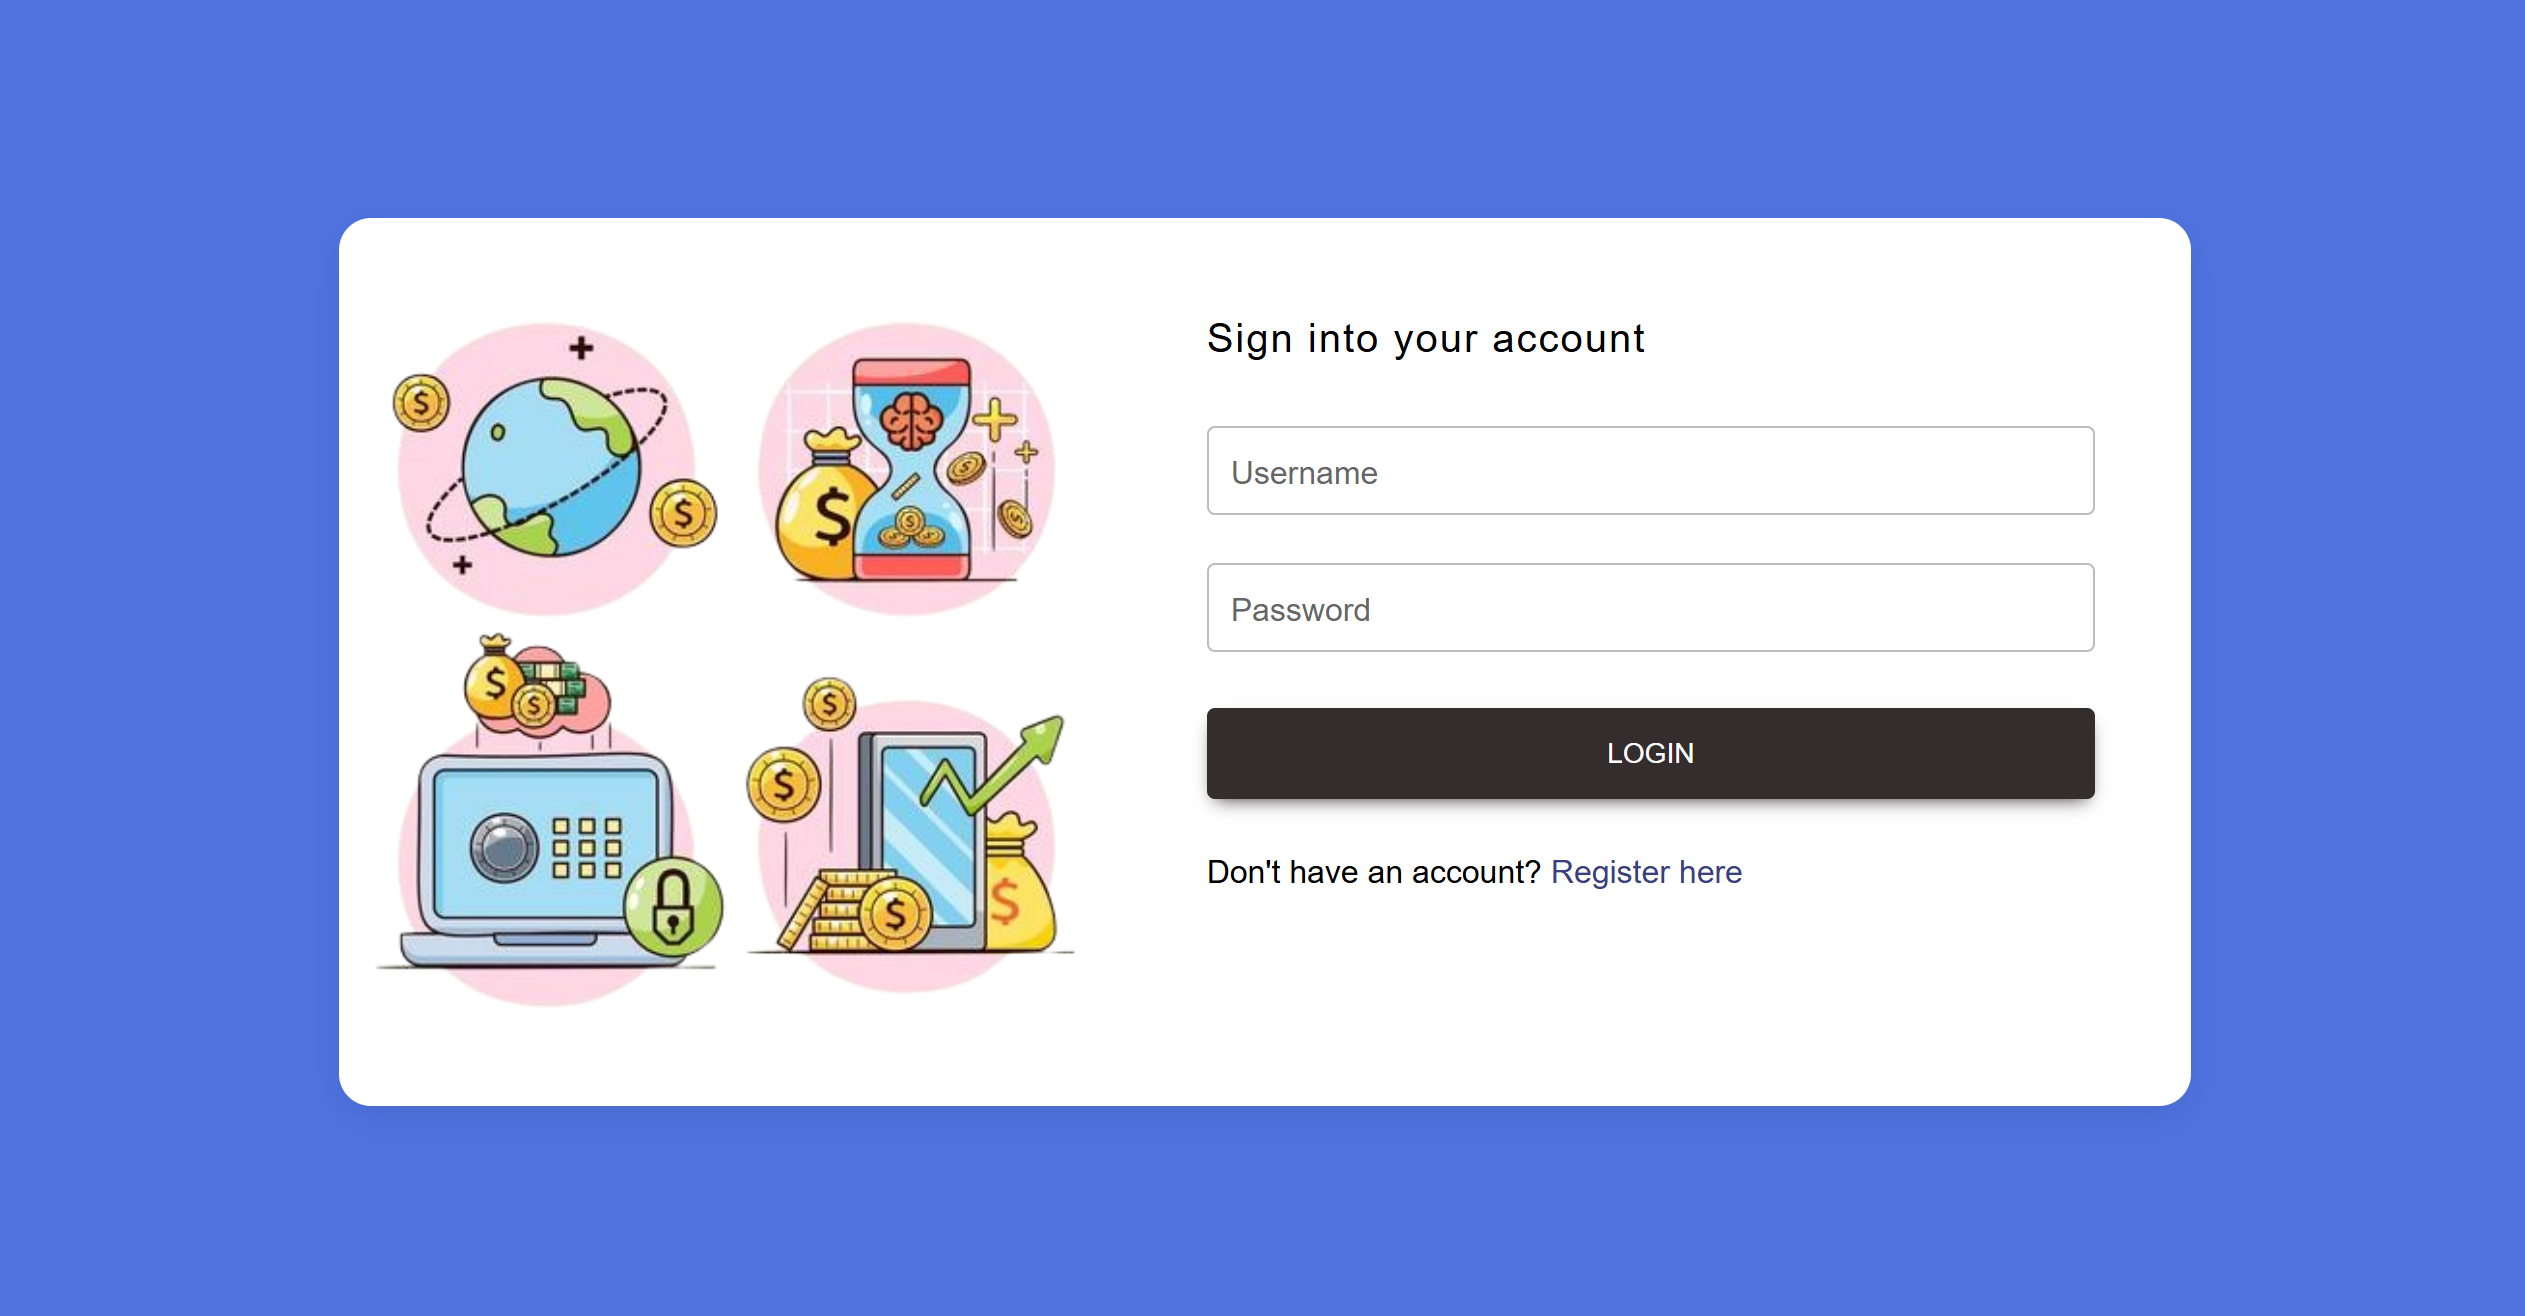
\includegraphics[height=180px]{img/login}
	\caption{Screenshot: Bejelentkező felület}
	\label{fig:login}
\end{figure}

\begin{figure}[H]
	\centering
	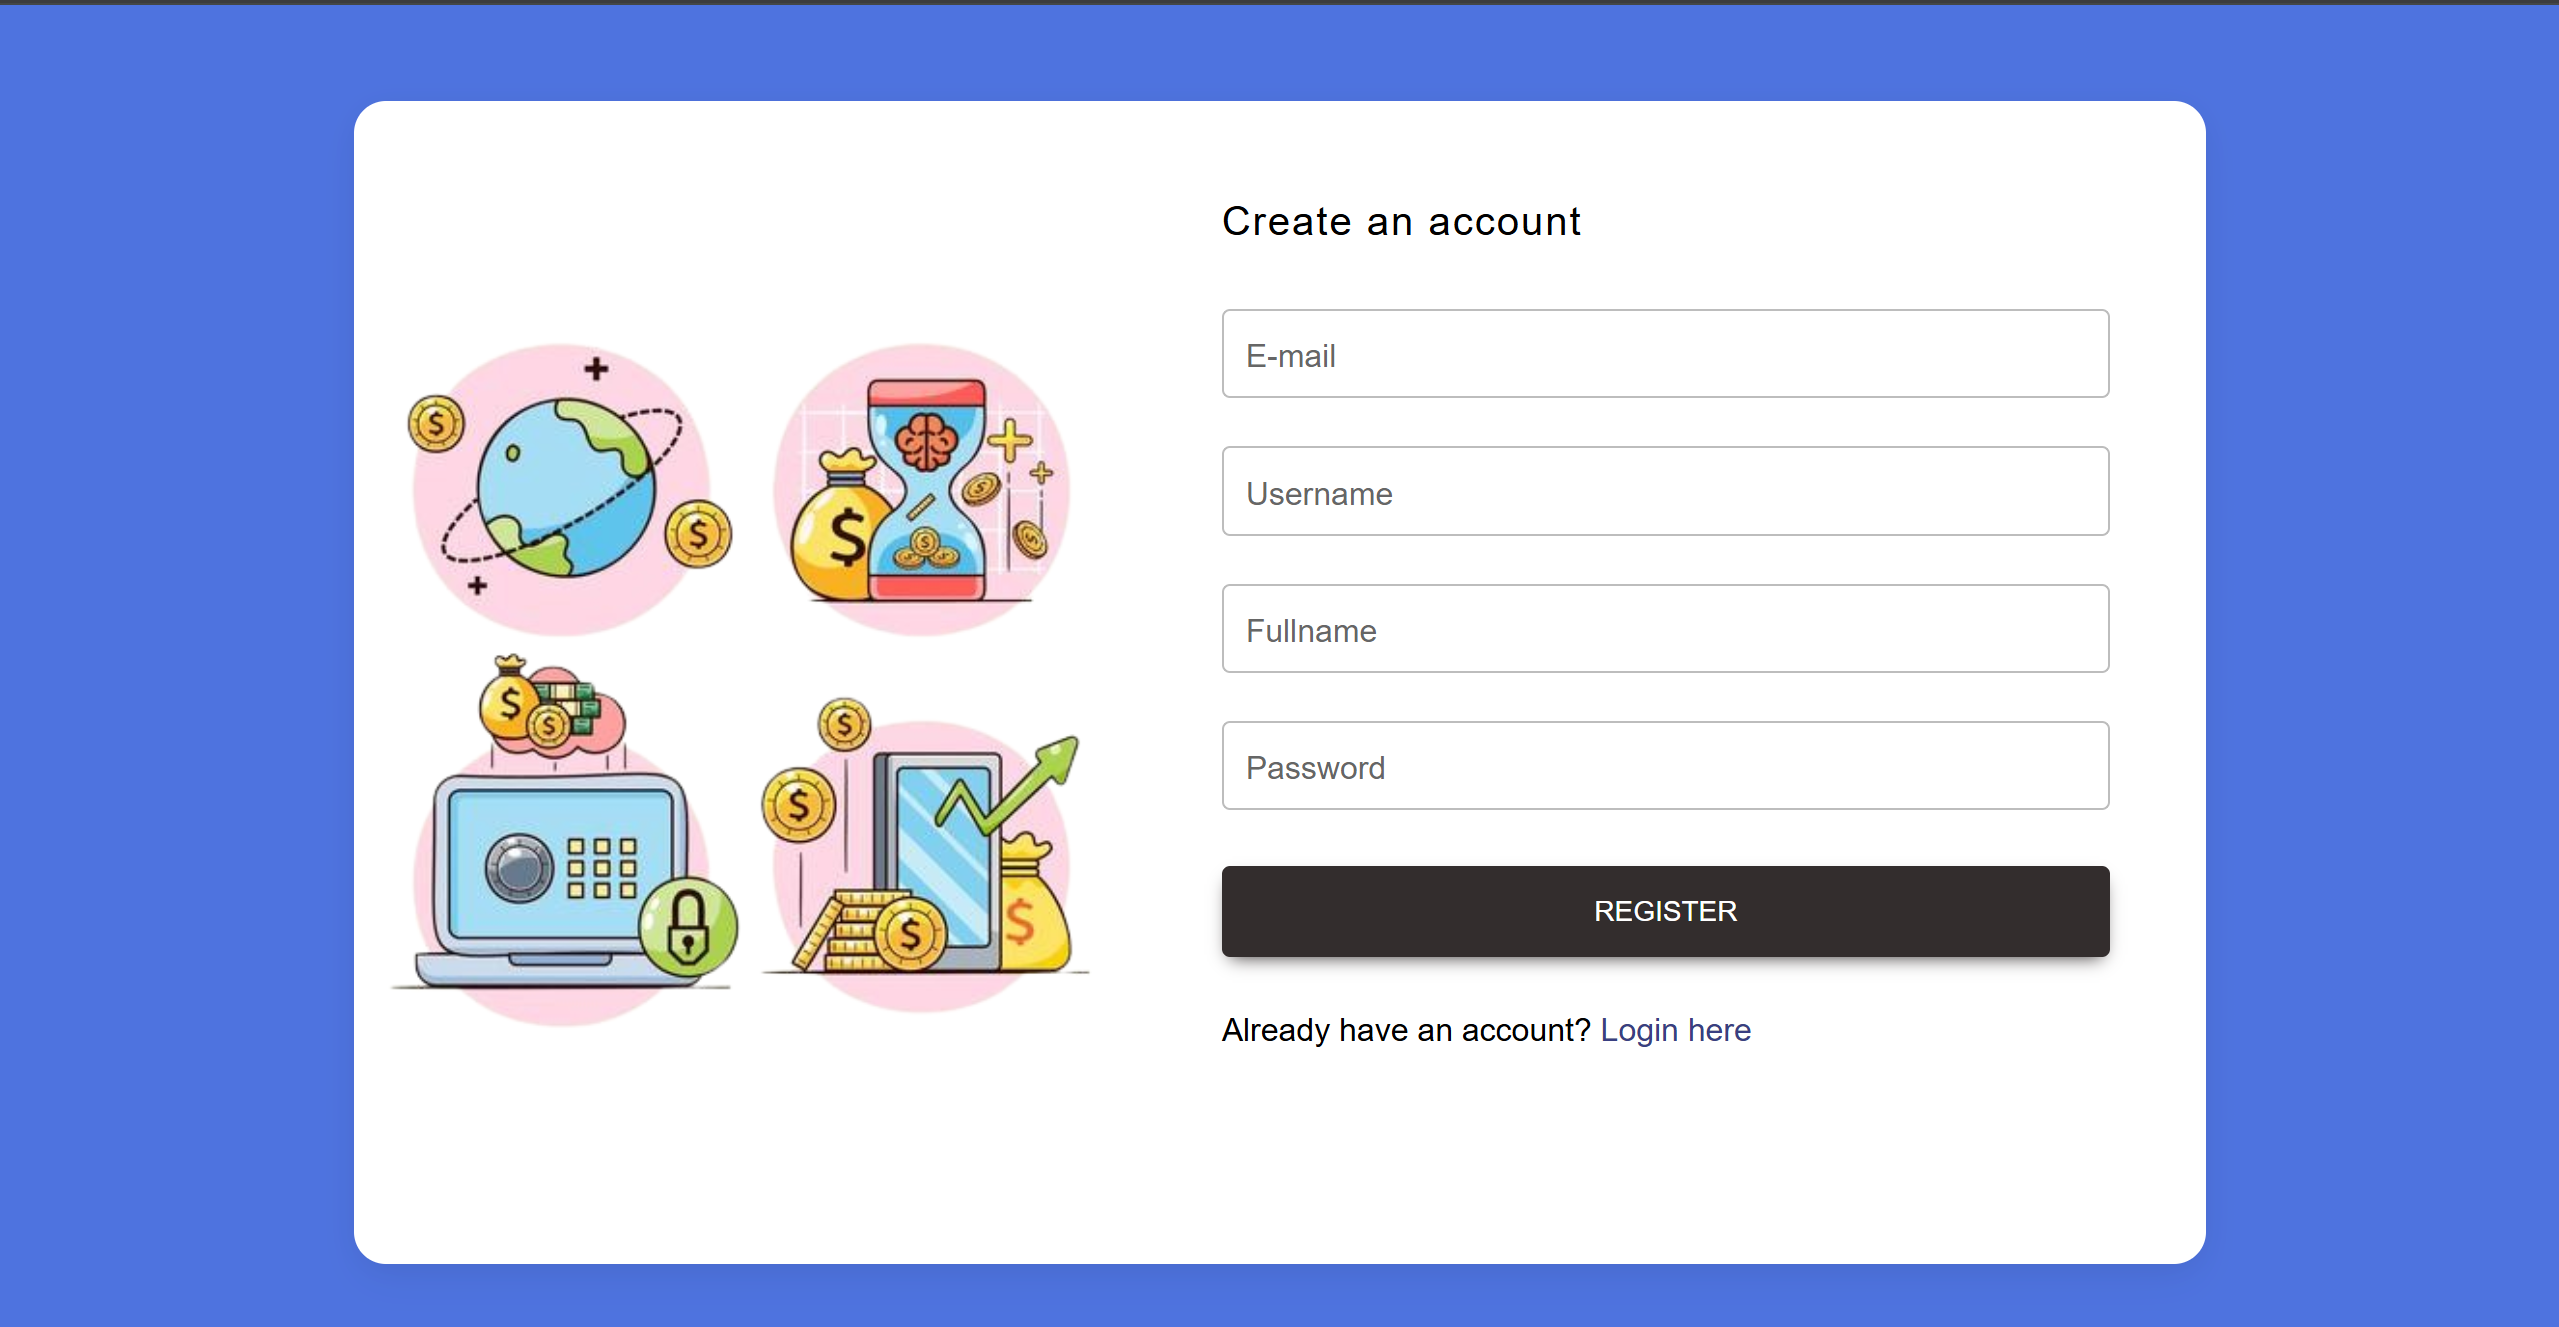
\includegraphics[height=180px]{img/register}
	\caption{Screenshot: Regisztrációs felület}
	\label{fig:register}
\end{figure}
\begin{table}[H]
	\centering
	\begin{tabular}{ | m{0.25\textwidth} | m{0.65\textwidth} | }
		\hline
		\textbf{Funkció} & \textbf{Leírás} \\
		\hline \hline
		\emph{Bejelentkezés} & Bejelentkezés egy egyedi felhasználónévvel és egy jelszóval lehetséges. (\ref{fig:login}. ábra) \\
		\hline
		\emph{Regisztráció} &  Regisztrálni lehet az oldalra a következő adatok megadásával: e-mail cím, felhasználónév (egyedi), teljes név, jelszó. (\ref{fig:register}. ábra)  \\
		\hline
		\emph{Profil} & A Profil oldalon lehet a fiókhoz tartozó adatokat módosítani: a felhasználónevet, a teljes nevet, illetve az e-mail címet is. Itt elérhető még egy "Change Pass" gomb is, amely elnavigálja a felhasználót a jelszó megváltoztató felületre. A profil oldal használatát a \ref{tab:profile}. táblázat fejti ki bővebben. (\ref{fig:profile}. ábra) \\
		\hline
		\emph{Jelszó módosítás} & A Profil oldalról lehet a jelszó változtató felületet elérni a "Change Pass" gomb megnyomásával. Itt meg kell adni a következő adatokat: régi jelszó, új jelszó, új jelszó megerősítése. \\
		\hline
		\emph{Kijelentkezés} & Ha a felhasználó befejezte kívánt tevékenységét, akkor a bal oldali menüsáv alján található "Logout" gomb megnyomásával tud kijelentkezni. A kijelentkező gomb még elérhető a jobb felső sarokban található ember ikonra kattintva legördülő menüben is. \\
		\hline
	\end{tabular}
	\caption{Fiók műveletek}
	\label{tab:account}
\end{table}

\begin{table}[H]
	\centering
	\begin{tabular}{ | m{0.25\textwidth} | m{0.65\textwidth} | }
		\hline
		\textbf{Funkció} & \textbf{Leírás} \\
		\hline \hline
		\emph{Adatok megtekintése} & A regisztrációnál megadott személyes adatait a felhasználó itt tekintheti meg. \\
		\hline
		\emph{Adatok módosítása} &  A személyes adatok módosítására is itt van lehetőség, egyszerű beviteli mezőkkel lehet módosítani a felhasználónevet (egyedi), teljes nevet és e-mail címet. A "Change" gombra kattintva előugrik egy beviteli mező egy "Save" és "Cancel" gombbal kiegészítve. Az előbbi megpróbálja végrehajtani a kért módosítást, és jelzi az esetlegesen fellépő hibát (érvénytelen e-mail cím, foglalt felhasználónév, stb.) a felhasználó felé.  \\
		\hline
		\emph{Jelszó módosítás} & Ha a felhasználó módosítani kívánja a jelszavát, akkor a "Change Password" gombra kattintva megjelenik egy új felület, három szerveren is validált jelszó beviteli mezővel (régi, új, új megerősítése). \\
		\hline
	\end{tabular}
	\caption{Profil oldal}
	\label{tab:profile}
\end{table}

\begin{figure}[H]
	\centering
	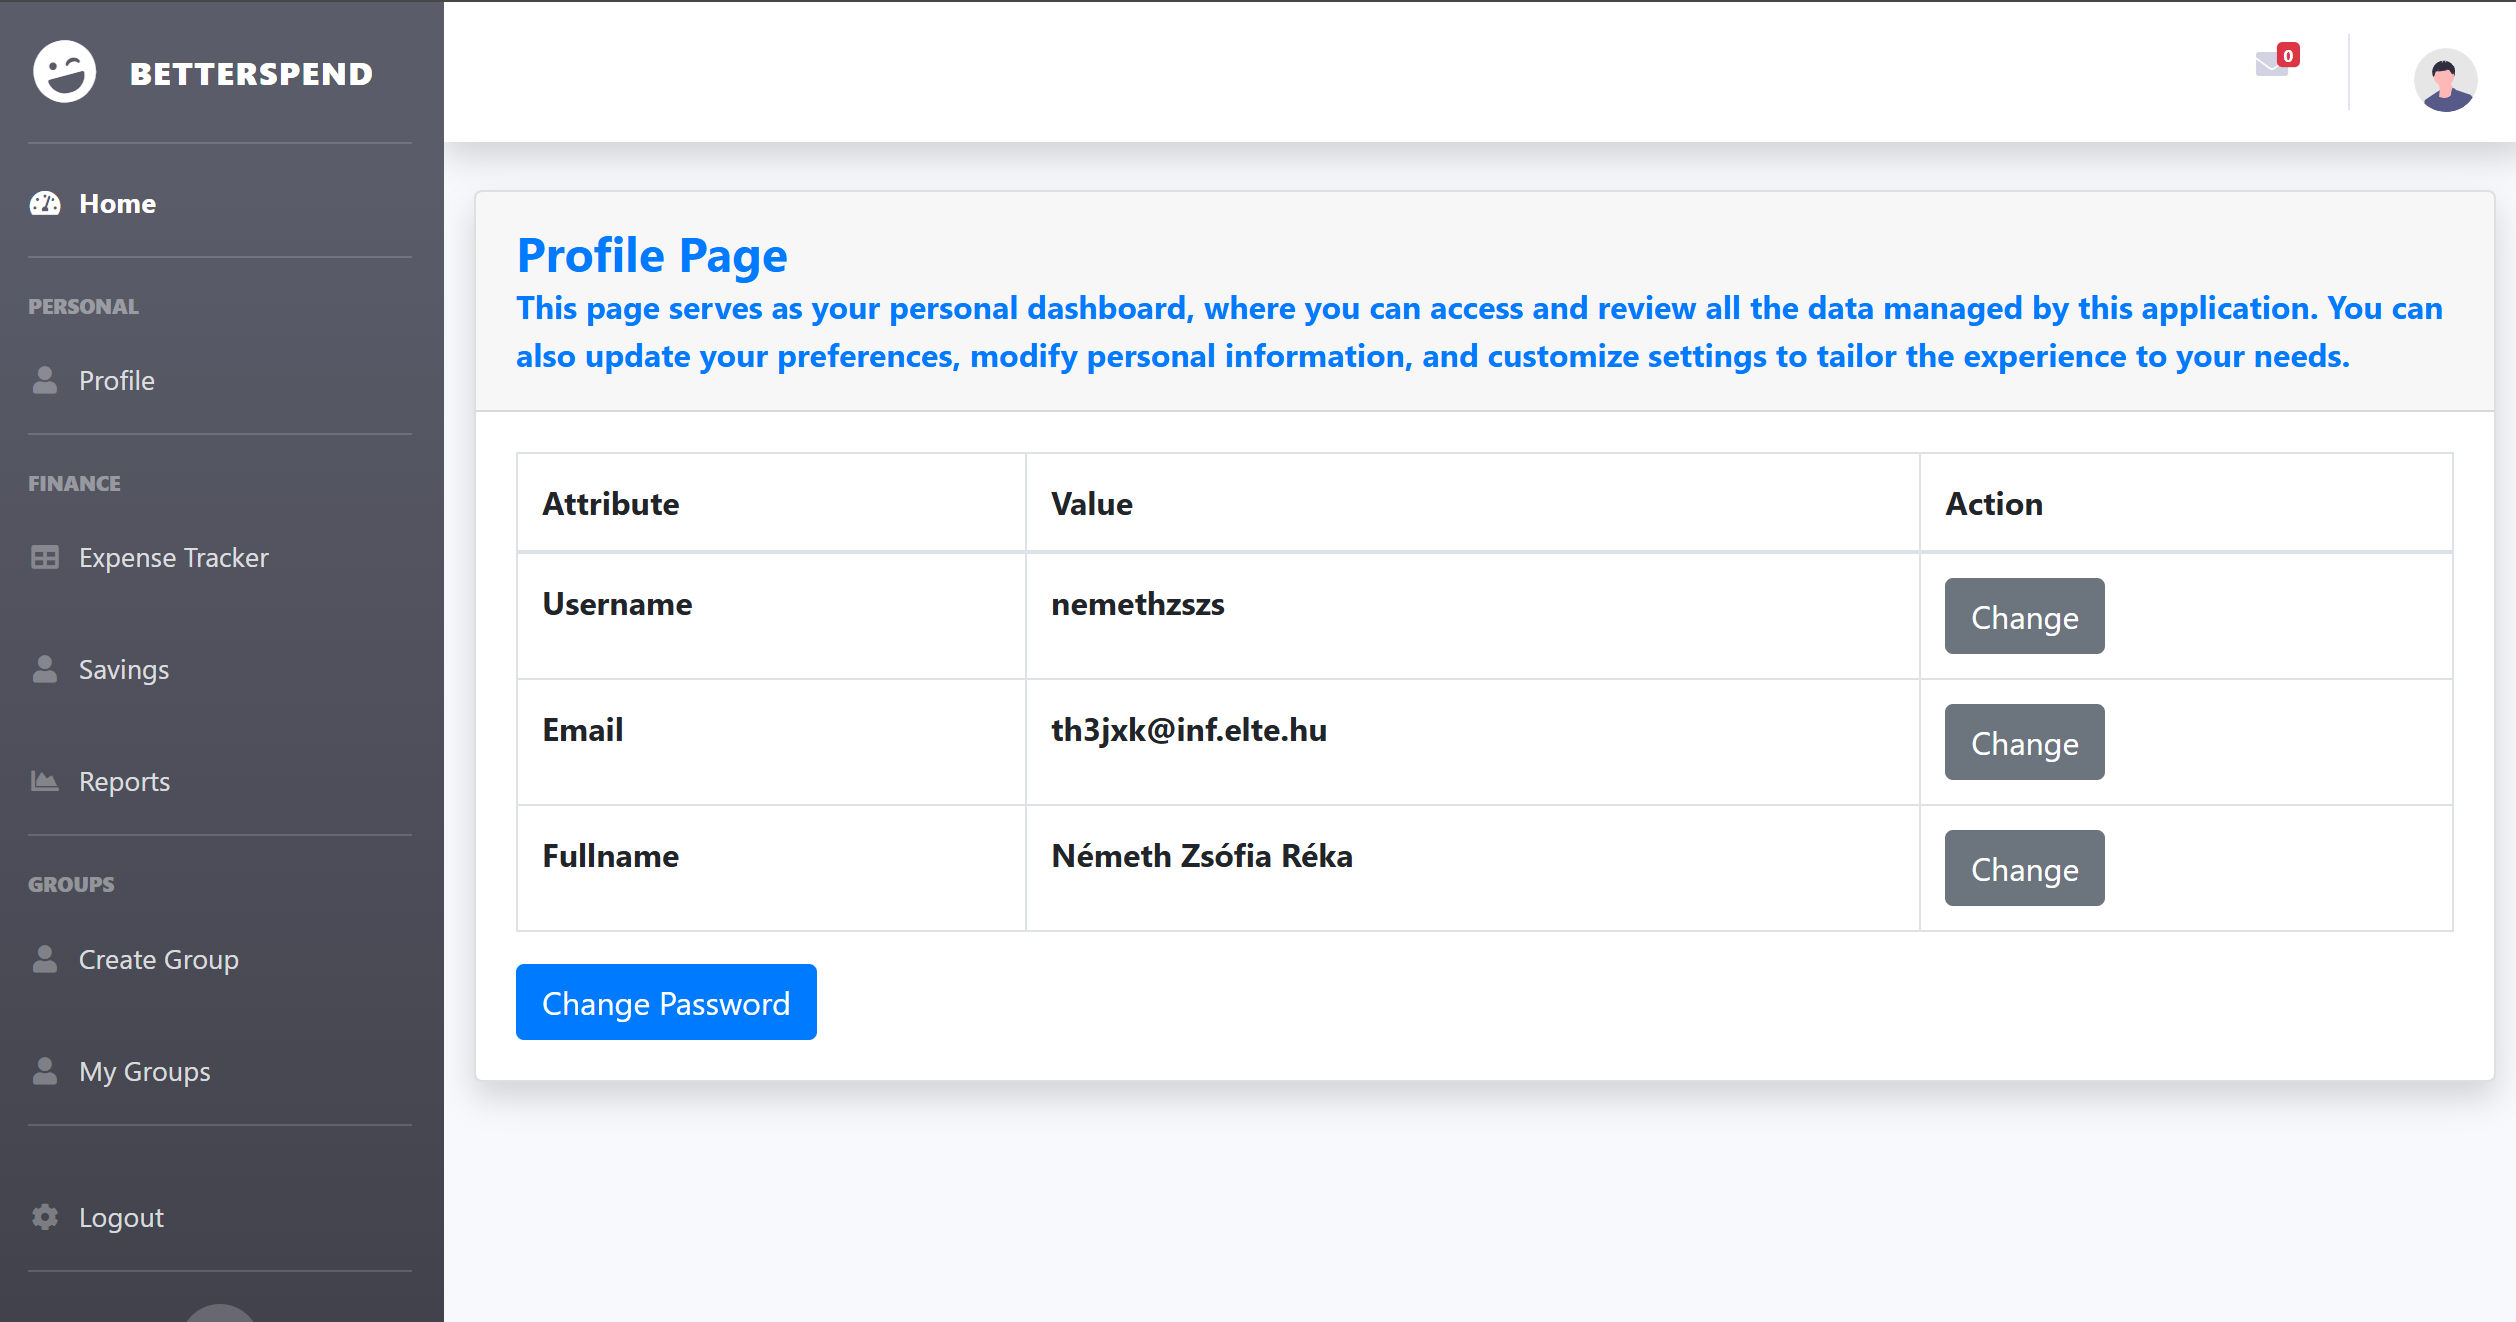
\includegraphics[height=190px]{img/profile}
	\caption{Screenshot: Profil felület}
	\label{fig:profile}
\end{figure}

\subsection{Pénzügyek}
A pénzügyeket kezelő oldalakat a kezdőképernyőről, illetve a baloldalon lévő menüből érhetjük el. A "Finance" cím alatt 3 különböző lap került kialakításra.
\begin{itemize}
	\item Tracker (\ref{tab:expense-tracker}. táblázat) (Bevételek és kiadások vezetése, és előzmények megtekintése)
	\item Savings (\ref{tab:savings}. táblázat) (Megtakarítások megtekintése és kezelése)
	\item Reports (\ref{tab:reports}. táblázat) (Kimutatások megtekintése, személyre szabása és exportálása) 
\end{itemize}

\subsubsection{Tracker felület}
A Tracker felület foglalja magában a bevételek és kiadások vezetését, illetve az előzmények megtekintését és korábbi tranzakciók eltávolítását.
\begin{table}[H]
	\centering
	\begin{tabular}{ | m{0.25\textwidth} | m{0.65\textwidth} | }
		\hline
		\textbf{Funkció} & \textbf{Leírás} \\
		\hline \hline
		\emph{Kiadás/bevétel rögzítése} & Külön dobozokban lehet rögzíteni a kiadásokat, és a bevételeket. Egyszerre egyet lehet bevinni, melynek adni kell egy összeget, egy leírást, opcionálisan lehet kategóriát is megadni. \\
		\hline
		\emph{Előzmények} &  A költési és bevételi előzményeket is itt lehet megtekinteni egy összesítő táblázatban. A táblázatban felül a "Search" mező módosításával lehet szűrni címszó alapján, azaz tudunk bármire (összegre, címre, kategóriára, stb.) keresni. Illetve az oszlopok címeire kattintva rendezni is lehet őket. A táblázat utolsó ("Delete") oszlopa arra szolgál, hogy egy adott sorban a kuka ikonra rákattintva, az a bejegyzés törlődik.  \\
		\hline
	\end{tabular}
	\caption{Tracker oldal}
	\label{tab:expense-tracker}
\end{table}

\subsubsection{Megtakarítás felület}
\begin{figure}[H]
	\centering
	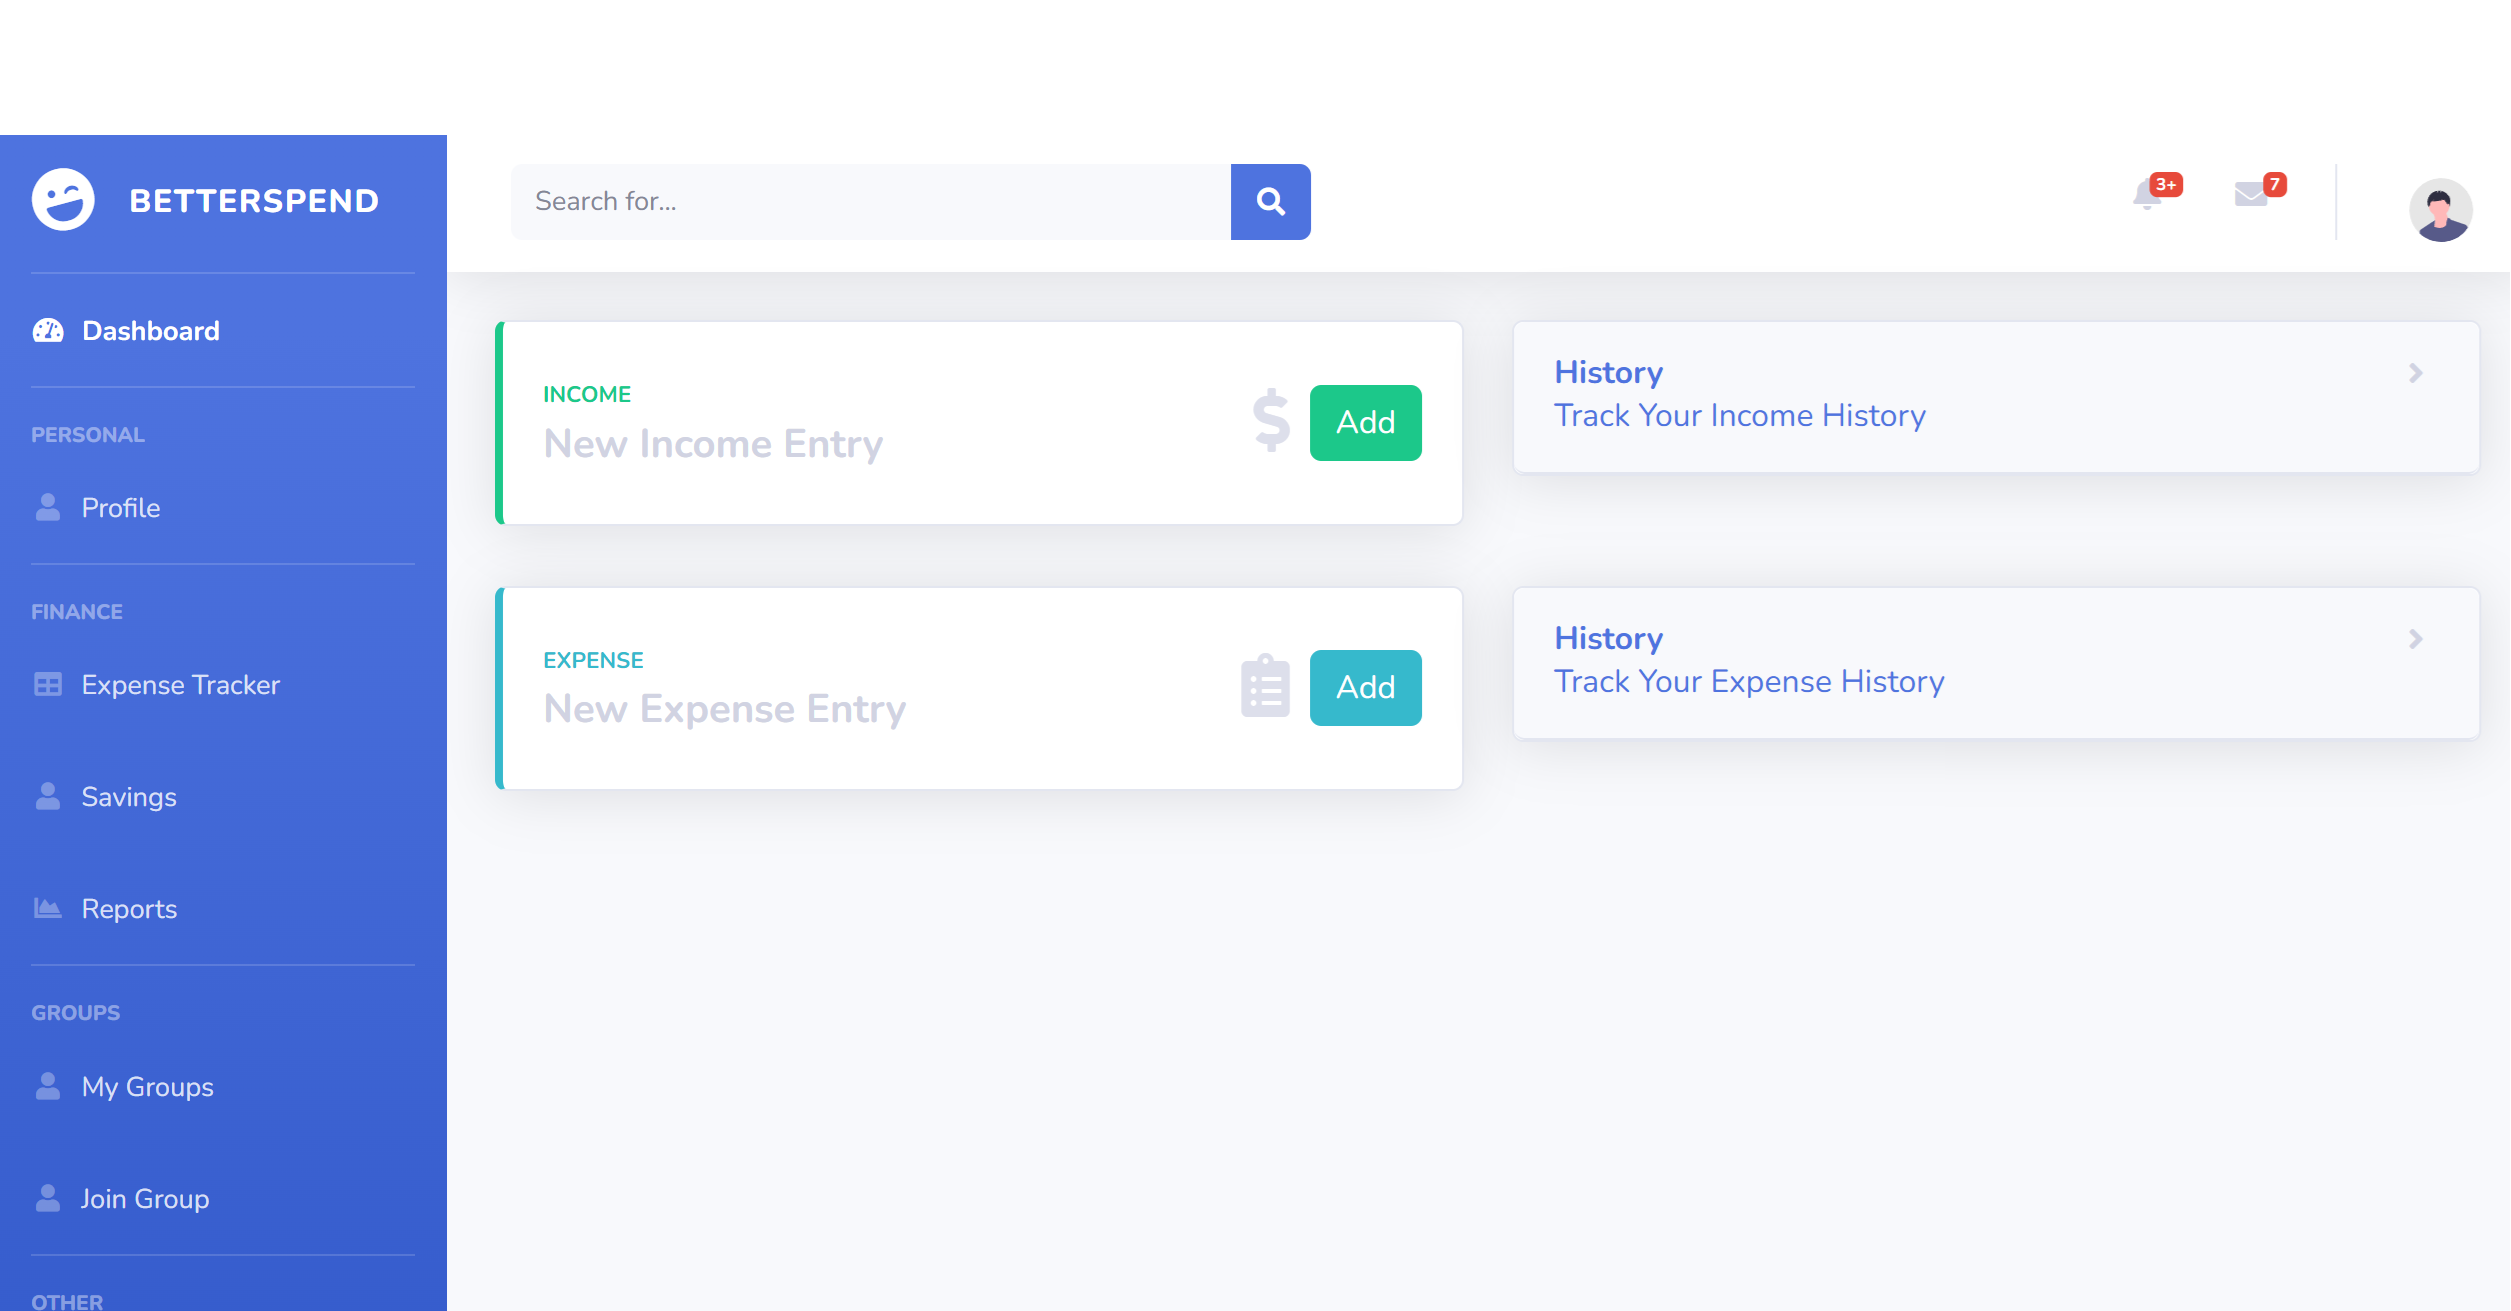
\includegraphics[height=190px]{img/expense-tracker-screenshot}
	\caption{Screenshot: Expense Tracker felület}
	\label{fig:expense-tracker}
\end{figure}

\begin{table}[H]
	\centering
	\begin{tabular}{ | m{0.25\textwidth} | m{0.65\textwidth} | }
		\hline
		\textbf{Funkció} & \textbf{Leírás} \\
		\hline \hline
		
		\emph{Új gyűjtés létrehozása} &
		A felhasználó új megtakarítási célt hozhat létre, például egy konkrét vásárlás vagy vészhelyzeti alap létrehozásához. A cél tartalmazhat megnevezést, opcionális leírást, célösszeget és határidőt. A cél a főoldalon egy külön kártyaként jelenik meg. \\
		
		\hline
		
		\emph{Összeg hozzáadása a gyűjtéshez} &
		Lehetővé teszi, hogy a felhasználó megtakarított összeget adjon hozzá egy kiválasztott célhoz. A kártyán található beviteli mező és "Add to Savings" gomb segítségével történik a művelet. Az aktuális megtakarítás értéke és a haladás százalékos formában is megjelenik. \\
		
		\hline
		
		\emph{Összeg kivonása a gyűjtésből} &
		Amennyiben a felhasználó el kíván távolítani egy összeget a gyűjtésből (pl. téves bevitel miatt), azt megteheti a "Withdraw" gomb segítségével. Ez a funkció csökkenti a gyűjtött összeget, de nem törli a célt. \\
		
		\hline
		
		\emph{Gyűjtés törlése} &
		A gyűjtés jobb felső sarkában elhelyezett kuka ikon segítségével a felhasználó teljesen eltávolíthat egy megtakarítási célt. Ez véglegesen törli az adott kártyát és a hozzá tartozó adatokat. \\
		
		\hline
		
		\emph{Cél elérése vizualizáció} &
		Ha a megtakarított összeg eléri vagy meghaladja a kitűzött célt, a kártya vizuálisan zöld színre vált. \\
		
		\hline
	\end{tabular}
	\caption{A Savings oldal}
	\label{tab:savings}
\end{table}
\begin{figure}[H]
	\centering
	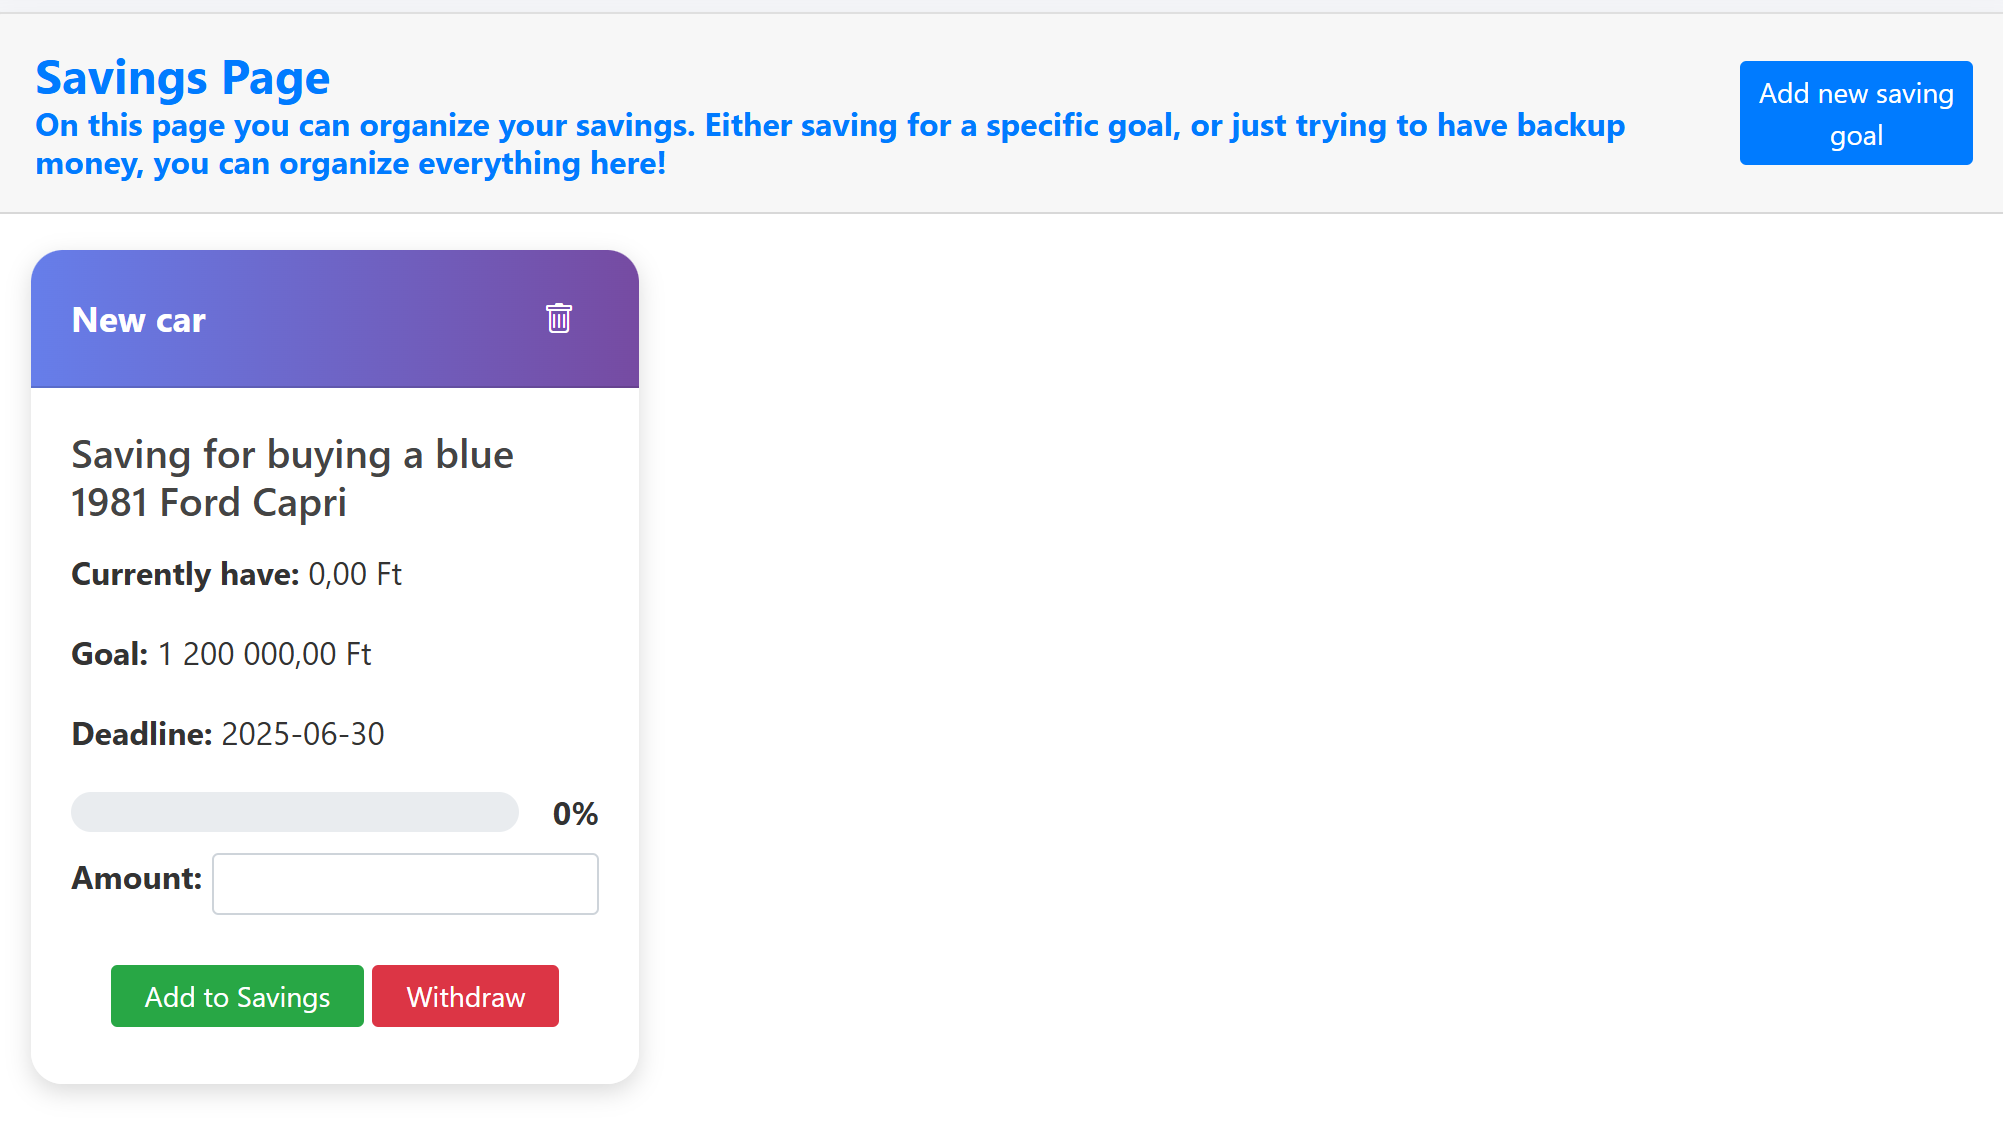
\includegraphics[height=190px]{img/savings}
	\caption{Screenshot: Savings felület}
	\label{fig:savings}
\end{figure}
\begin{figure}[H]
	\centering
	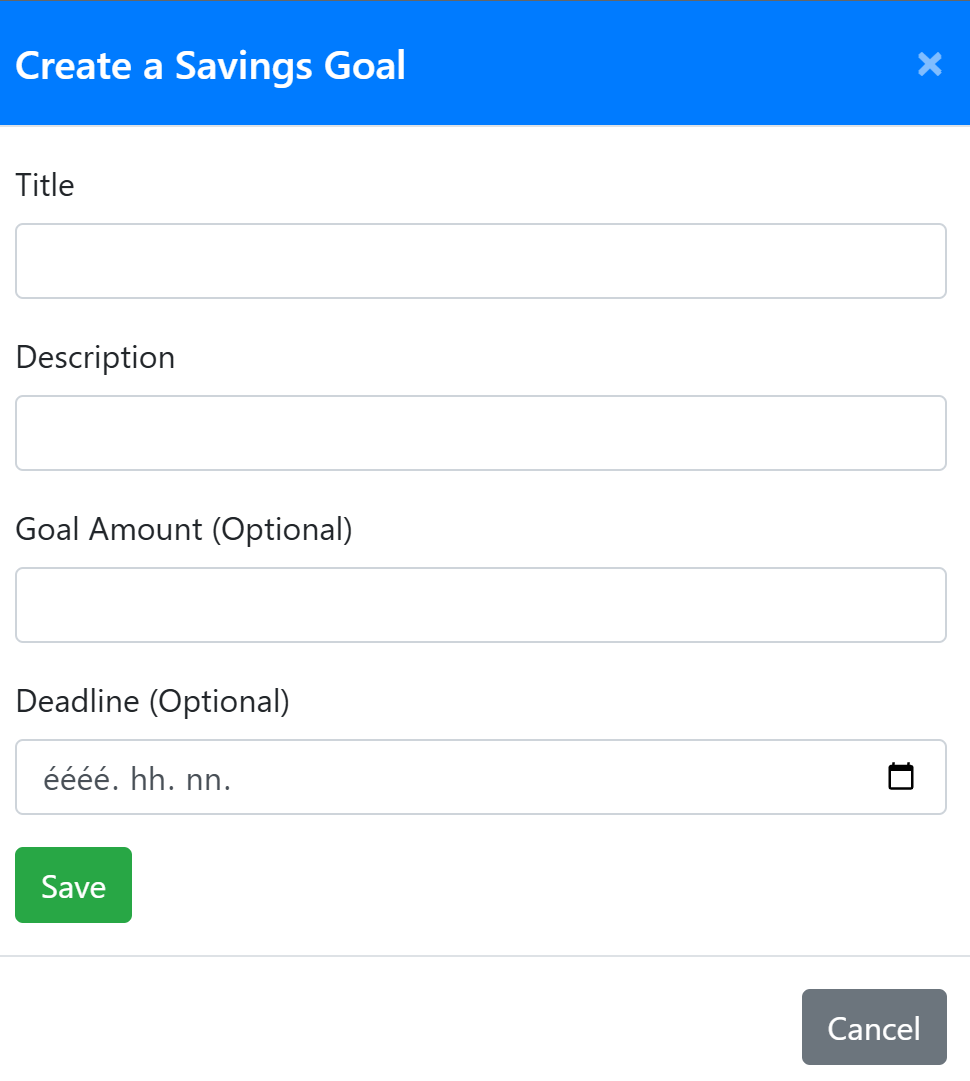
\includegraphics[height=190px]{img/add-saving}
	\caption{Screenshot: Gyűjtés létrehozása}
	\label{fig:addsaving}
\end{figure}

\subsubsection{Kimutatások felület}
\begin{table}[H]
	\centering
	\begin{tabular}{ | m{0.25\textwidth} | m{0.65\textwidth} | }
		\hline
		\textbf{Funkció} & \textbf{Leírás} \\
		\hline \hline
		
		\emph{Havi kimutatás} &
		Az oldal első szekciója egy vonaldiagramot jelenít meg, amely napi bontásban mutatja az adott hónap bevételeit és kiadásait. A diagram segít a felhasználónak átlátni a pénzmozgásokat, észrevenni a kiugró értékeket. A színek jól elkülönítik a bevételt (zöld) és a kiadást (piros). \\
		
		\hline
		
		\emph{Részletes jelentés letöltése} &
		Egy letöltés gomb lehetőséget ad arra, hogy a felhasználó exportálja a részletes pénzügyi riportot (pl. PDF vagy CSV formátumban). Ez hasznos lehet adminisztrációhoz vagy év végi összesítéshez. \\
		
		\hline
		
		\emph{Éves összehasonlító jelentés} &
		Az oldal alsó részén található oszlopdiagram összehasonlítja az egyes hónapok bevételi és kiadási értékeit. A felhasználó egy legördülő listából kiválaszthatja az évet (pl. 2025), amely alapján frissül a diagram. Ez segít az éves pénzügyi trendek nyomon követésében. \\
		
		\hline
		
		\emph{Vizualizáció és színkódolás} &
		A grafikonok színkódolása konzisztens az alkalmazás többi részével: zöld a bevételre, piros a kiadásra utal. A jól strukturált vizualizáció megkönnyíti az adatok gyors értelmezését, különösen a visszatérő pénzügyi mintázatok felismerését. \\
		
		\hline
	\end{tabular}
	\caption{A Reports oldal funkciói és működése}
	\label{tab:reports}
\end{table}

\subsection{Csoportok}
A csoportokban leginkább ugyanazok a funkciók találhatóak, melyek a személyes használat esetében is. Ezeket az előző fejezetek taglalták részletesebben.
\begin{table}[H]
	\centering
	\begin{tabular}{ | m{0.25\textwidth} | m{0.65\textwidth} | }
		\hline
		\textbf{Funkció} & \textbf{Leírás} \\
		\hline \hline
		\emph{-} & - \\
		\hline
	\end{tabular}
	\caption{Groups oldal}
	\label{tab:groups}
\end{table}

\begin{table}[H]
	\centering
	\begin{tabular}{ | m{0.25\textwidth} | m{0.65\textwidth} | }
		\hline
		\textbf{Funkció} & \textbf{Leírás} \\
		\hline \hline
		\emph{-} & - \\
		\hline
	\end{tabular}
	\caption{My Groups oldal}
	\label{tab:my-groups}
\end{table}